\documentclass[12pt]{article}

\usepackage{sbc-template}

\usepackage{graphicx,url}

\usepackage[brazil]{babel}   
%\usepackage[latin1]{inputenc}  
\usepackage[utf8]{inputenc}  
% UTF-8 encoding is recommended by ShareLaTex

     
\sloppy

\title{Um método crowdsourcing para geração de objetos de aprendizagem por meio do enriquecimento de vídeos}


\author{Marcello N. Amorim\inst{1}, Celso A. S. Santos\inst{2}, Orivaldo L. Tavares\inst{3} }


\address{Programa de pós-graduação em Informática -- Universidade Federal do Espírito Santo
  (UFES)\\
  Av. Fernando Ferrari, 514, CEP 29075-910, Goiabeiras -- Vitória, ES -- Brasil
  \email{\{novaes,saibel,tavares\}@inf.ufes.br}
}

\begin{document} 

\maketitle

\begin{abstract}
This article introduces a method for generating learning objects based on video enrichment. The proposed method allows to identify information gaps that can occur in educational videos and fill them with complementary content by aggregating multimedia artifacts such as images, text boxes, or interactive features such as hyperlinks. This method is supported by a computational environment, which facilitates the use of a hybrid approach. In this approach, the identification of semantic gaps, the obtaining of information to generate the complementary content, and the validation of the generated content, are carried out by the students themselves in a crowdsourcing approach, while the multimedia artifacts that are added to the videos are generated by automatic techniques from the students' contributions. The goal of this work is to generate learning objects based on educational videos that are more effective than the original videos as didactic material. The research question is whether the learning objects generated are actually didactic material superior to the original videos, and this verification is done through the practical experience which is also detailed in this article.
\end{abstract}
     
\begin{resumo} 
\input{topicos/resumo}
\end{resumo}

\pagebreak

\section{Introdução}
A utilização de vídeos como objetos de aprendizagem é uma prática já consolidada, e que cresce continuamente na medida em que as câmeras e \textit{smartphones} se tornam mais acessíveis, e as plataformas de distribuição como \textit{Youtube} e \textit{Vimeo} se popularizam  \cite{Davis:2015:YoutubeVimeo}. Todavia, o modelo clássico de produção de vídeos, que ainda é predominante atualmente, é um modelo centralizado que contempla apenas o ponto de vista do autor. O resultado deste processo focado em um ponto de vista único é a ocorrência de lacunas semânticas no vídeo \cite{Bhimani:2013:VPE:2465958.2465976}. 

Estas lacunas semânticas se caracterizam pela falta de informação necessária para que o estudante compreenda o conteúdo, com riqueza de detalhes. Elas ocorrem tanto nos casos em que o material didático realmente não oferece informação suficiente, quanto nos casos em que a maneira como a informação é apresentada não é adequada para aquele estudante. As lacunas semânticas em vídeos educacionais podem surgir por diversos motivos, e inevitavelmente geram problemas de compreensão, resultando em uma menor eficiência do vídeo como material didático. Neste trabalho serão abordados três tipos de lacunas semânticas: 
\begin{itemize}
    \item Termos e expressões de compreensão que podem não ser compreendidos;
    \item Conceitos que necessitam de explicações ou definições adicionais;
    \item Fatos e afirmações que precisam ser contextualizados.
\end{itemize}


Este trabalho apresenta um método para preencher as lacunas semânticas em vídeos educacionais por meio da agregação de artefatos multimídia que contenham informações adicionais. Este método também permite aprimorar a interação do estudante com o vídeo, adicionando recursos que melhorem a navegação e o acesso à informação contida neles. Existem diversos tipos de artefato multimídia e recursos interativos que podem ser agregados aos vídeos. Neste trabalho serão utilizados imagens, caixas de mensagem e hiperlinks.

O método proposto permite que o processo de enriquecimento, que consistem em gerar os artefatos multimídia e recursos interativos para então agrega-los ao vídeo, seja realizado sem a necessidade de profissionais experientes ou equipamentos e sistemas caros. Para tal, é utilizada uma abordagem \textit{Crowdsourcing} \cite{Howe2006} para coletar contribuições dos próprios estudantes, e determinar as informações usadas para gerar o conteúdo extra a ser agregado ao vídeo. Este método utiliza uma estratégia híbrida para gerar automaticamente o conteúdo extra, com base nas informações geradas a partir das contribuições dos estudantes.

O objetivo do método é gerar objetos de aprendizagem baseados em vídeos educacionais, que sejam mais eficientes como material didático que os vídeos originais. A questão de investigação deste trabalho, de forma complementar, é verificar se o método proposto pode realmente gerar objetos de aprendizagem que sejam mais eficazes que o vídeo original como material didático.

O restante do artigo apresenta-se da seguinte forma: a Seção 2 trata das lacunas semânticas em vídeos, suas causas e efeitos; na Seção 3 são justificadas e descritas a abordagem do problema, a estratégia de solução e as técnicas utilizadas; na Seção 4 é detalhado o método proposto; na Seção 5 é apresentado o ambiente de apoio ao método; na Seção 6 é apresentado o estudo de caso, com o experimento prático realizado e análise dos seus resultados; e finalmente, na Seção 7 são feitas as considerações finais.




\section{Lacunas Semânticas}
Lacunas semânticas são falhas de informação que dificultam a extração de informação útil do fluxo de vídeo este problema é tratado com frequência nos trabalhos relacionados com segmentação de imagens e identificação de objetos de cenas \cite{895972,SnoekICM2005}. Um exemplo clássico de lacuna semântica neste contexto é a oclusão de parte de um objeto: se em uma cena não se pode ser as mãos de um personagem, então não se pode identificar o que ele está segurando. Este mesmo conceito pode ser aplicado no contexto dos vídeos educativos, em um cenário no qual são os que estudantes precisam extrair informação útil do fluxo de vídeo.

As pessoas são capazes de preencher algumas lacunas semânticas por meio de inferências, associações com seu conhecimento prévio e o contexto identificado. Desta forma, cada indivíduo tem sua própria limitação em relação a quais lacunas é capaz de preencher. Isso significa que apesar de as lacunas semânticas contidas em um vídeo serem as mesmas, pessoas com diferentes características são afetadas por cada uma dela com intensidades diferentes.

No modelo clássico de produção de vídeo, que é utilizado de forma predominante, tudo é direcionado para o ponto de vista do autor. Isso significa que todas as cenas capturadas, conteúdo representado, e mesmo a forma como as informações são transmitidas, são determinados pelo que o autor quis mostrar e da forma como ele quis mostrar \cite{Bhimani:2013:VPE:2465958.2465976}. O problema neste processo é que o autor pode não perceber, no vídeo, as lacunas semânticas que ele é capaz de preencher, mas que podem causa sérios problemas de compreensão para outras pessoas que assistam ao vídeo. 

Estas lacunas semânticas em vídeos educacionais podem ocorrer sempre que um estudante não pode compreender parte do conteúdo por sentir falta de informação sobre ela. Elas podem acontecer mesmo quando a informação está presente no vídeo, caso ela não seja apresentada de uma forma que o estudante possa compreender, por exemplo, quando ele acessa um vídeo que está em um idioma que ele desconhece. 

São diversas as causas deste tipo de lacuna semântica, todavia foram selecionadas três delas para serem abordadas neste projeto. A primeira causa é ocorrência de expressões e termos que podem não ser compreendidos corretamente pelo estudante. Este problema está diretamente relacionado com os regionalismos e termos técnicos. A segunda causa diz respeito aos conceitos que são apresentados ao estudante, mas que precisam se melhor explicados ou exemplificados para que ele os compreenda. A terceira causa é a falta de contextualização ao se apresentar um fato. Isso ocorre quando se apresenta uma afirmação ao estudante, mas não se diz em quais condições aquele fato ocorreu, ou é válido.


\section{Abordagem do Problema}
O enriquecimento dos vídeos educacionais, da forma como é proposto neste trabalho, envolve uma série de questões desafiadoras:
\begin{enumerate}
    \item A detecção das lacunas semânticas é uma tarefa que depende da percepção dos estudantes;
    \item O conteúdo utilizado para preencher as lacunas deve satisfazer os estudantes;
    \item Mesmo vídeos curtos requerem muito esforço para serem analisados, pois existe muita informação concentrada em cada segmento;
    \item As atividades de geração de conteúdo complementar multimídia, e de agregação deste conteúdo ao vídeo, requerem uma quantidade grande de esforço e recursos;
\end{enumerate}


Para superar estas dificuldades foram selecionadas algumas técnicas que, em conjunto, permitem que o enriquecimento de vídeos seja feito de maneira colaborativa, e que os estudantes possam contribuir realizando apenas atividades que realmente necessitem de inteligência humana.

O paradigma de computação humana ajuda a modelar cenários nos quais parte das atividades devem ser realizadas por pessoas e a outra parte pode ser executada por meios automáticos \cite{VonAhn:2005:HC:1168246}. Sendo assim, este ponto de vista se mostra totalmente compatível com o enriquecimento de vídeos educativos, uma vez que as atividades de identificação das lacunas semânticas e obtenção das informações necessárias para cobri-las requerem inteligência humana, e a geração e agregação dos artefatos multimídia são atividades que podem ser automatizadas.

Um ponto positivo da computação humana é a possibilidade de paralelizar as atividades que requerem inteligência humana, desta forma é possível agilizar o processo de coleta das contribuições.  Todavia, para que este modelo seja aplicado neste trabalho é necessário que estas atividades sejam modeladas corretamente, e que sejam distribuídas de maneira eficiente entre os estudantes. Nestas condições, uma abordagem crowdsourcing baseada em micro-tarefas se mostra muito adequada para distribuir, coletar e gerenciar as tarefas e contribuições \cite{Difallah:2015:DMC:2736277.2741685}. Neste tipo de abordagem, uma série de pequenas tarefas é distribuída entre os colaboradores, gerando uma base de resultados parciais que são validados, filtrados e agregados, permitindo que se gere um resultado final a partir das contribuições.

Com base em trabalhos relacionados, uma maneira eficiente de modelar as micro-tarefas, em sistemas crowdsourcing que visam gerar artefatos sobre vídeos, é como tarefas de anotação \cite{ref:vidwiki2014,Wu:2011:VSV:1979742.1979803}. As anotações são meta-informações relacionadas com um artefato, e podem representar diferentes características dele tanto em relação à sua forma, quanto ao seu conteúdo \cite{Singhal:2014:GSA:2611040.2611056}. Neste projeto, as anotações sobre os vídeos serão utilizadas para representar as contribuições dos estudantes. Em outras palavras, para cada tarefa executada por um estudante será coletada uma anotação que irá relacionar a contribuição com o segmento de vídeo ao qual ela diz respeito. Este tipo de tarefa pode ser modelada e executada de forma muito simples, podendo ser realizada pelos estudantes enquanto assistem ao vídeo.

Uma vez que as contribuições sejam coletadas dos estudantes por meio das tarefas de anotação, elas são validadas e processadas de acordo com um conjunto de filtros e técnicas de agregação já consolidadas em sistemas crowdsourcing \cite{Alelyani:2016:SCR:2989238.2989245,Hipp:2013}. O resultado final do processo colaborativo é uma base consolidada de informações, que representam aquilo que deve ser adicionado em cada segmento do vídeo, para que as lacunas semânticas sejam preenchidas. Como estas informações são coletadas dos estudantes, este preenchimento tente a gerar resultados que são satisfatórios para eles.

Uma vez que se tenha estas informações, a geração dos artefatos multimídia, irão representar o conteúdo complementar que deve ser adicionado ao vídeo, é feita por meio de técnicas automáticas baseadas em modelos. Estas técnicas utilizam modelos pré-determinados para cada tipo de artefato que pode ser instanciado, e conforme os atributos de são preenchidos estes objetos multimídia são criados. Finalmente, uma vez que o conteúdo extra esteja pronto, ele é alinhado sobre o vídeo, e agregado a ele de acordo com suas características.


\section{Método Proposto}
O método proposto segue um modelo híbrido para gerar objetos de aprendizagem por meio da agregação de artefatos multimídia em vídeos educacionais. Este método combina técnicas automáticas para geração de objetos multimídia com uma abordagem crowdsourcing para utilizar de forma eficiente as contribuições dos estudantes.

\begin{figure}[ht]
\centering
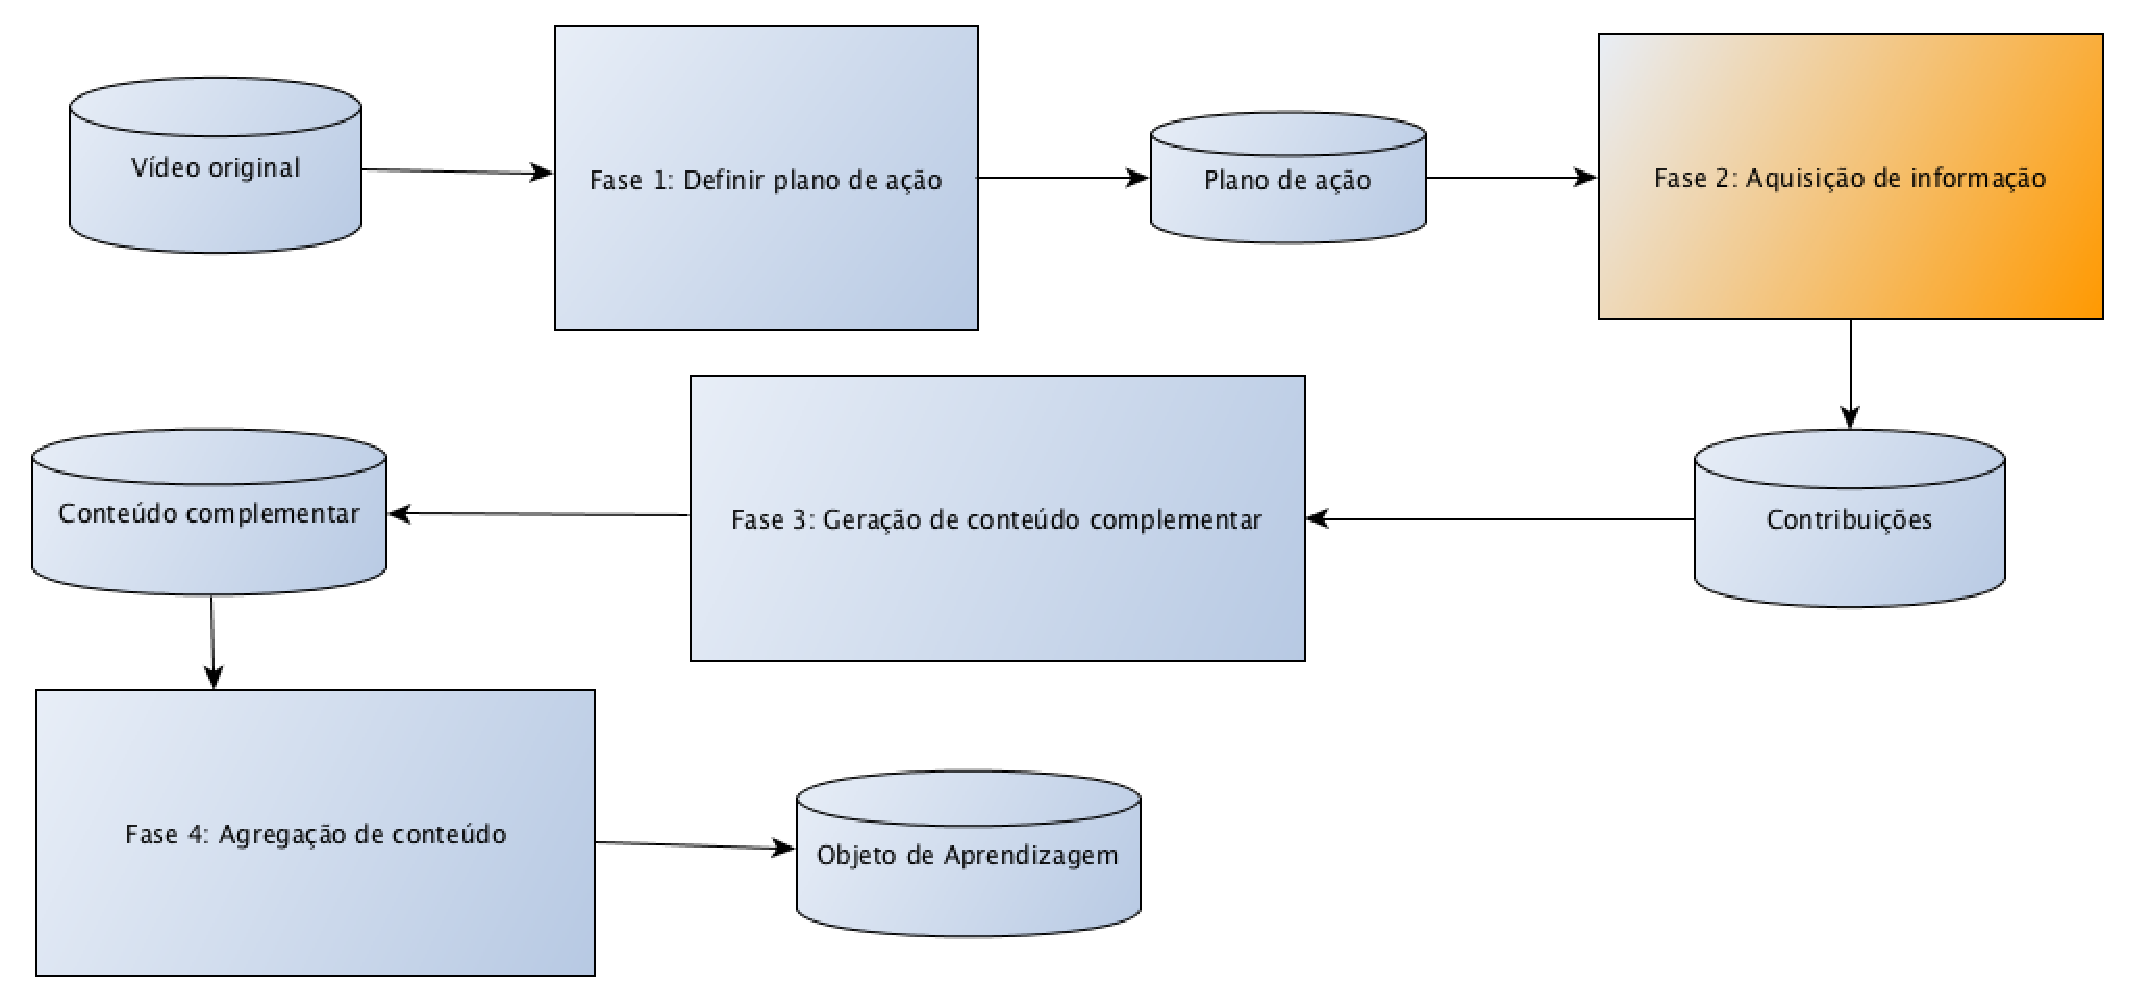
\includegraphics[width=.99\textwidth]{imagens/metodo/geral_oa.eps}
\caption{Visão geral do método}
\label{fig:metodo:geral}
\end{figure}


Conforme pode ser observado na Figura~\ref{fig:metodo:geral}, o método estabelece um processo para o enriquecimento do vídeo original, que resulta em um objeto de aprendizagem.

De forma resumida, o processo é realizado da seguinte maneira: inicialmente são definidas as características do objeto de aprendizagem a ser gerado, e a criação do plano de ação que deve ser seguido a fim de produzir o objeto de aprendizagem correto. Uma que o plano de ação está definido, tem inicio o processo crowdsourcing que utiliza as contribuições dos estudantes para determinar quais são as informações que devem ser utilizadas para gerar o conteúdo complementar. Após a coleta e processamento das contribuições, têm inicio a geração automática dos artefatos multimídia que serão agregados ao vídeo original. Por fim, após todos os artefatos estarem prontos, se faz o alinhamento deles sobre a linha do tempo do vídeo para que eles possam ser exibidos nos momentos corretos.












\subsection{Papeis}
Neste método existem três papeis que são desempenhados pelos envolvidos:
\begin{itemize}
    \item Iniciador: quem inicia o processo de enriquecimento e define as características do objeto de aprendizagem.
    \item Estudante: os estudantes são os colaboradores, eles compõem a multidão (crowd) utilizada nas atividades crowdsourcing.
    \item Sistema: o sistema assume o papel de um ator que realiza as atividades relacionadas com as técnicas automáticas.
\end{itemize}

\subsection{Fase 1: Definição do Plano de Ação}
A primeira fase é destinada a definir o plano de ação que deve ser seguido durante o restante do processo. Todas as atividades desta fase são realizadas pelo Iniciador, que é quem define as características do objeto de aprendizagem a ser gerado, e do processo de colaboração.

\begin{figure}[ht]
\centering
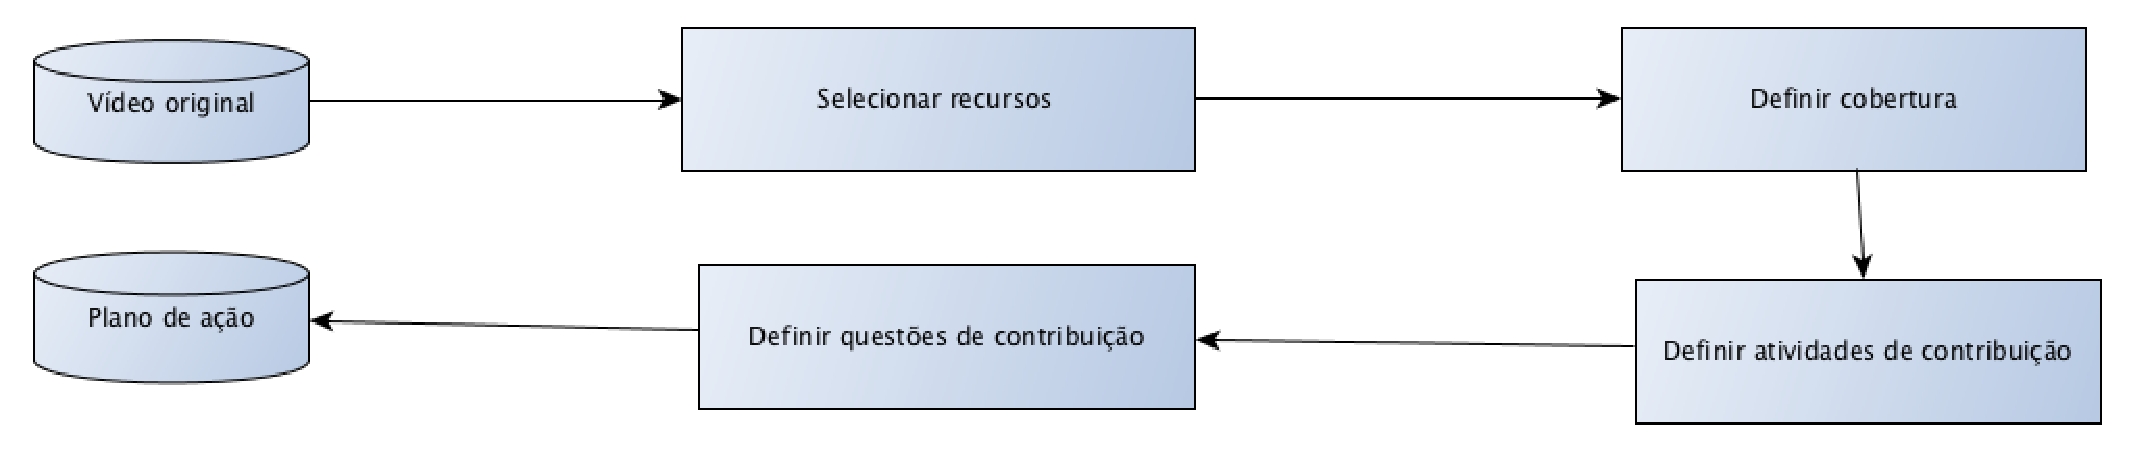
\includegraphics[width=.99\textwidth]{imagens/metodo/fase1_oa.eps}
\caption{Fase 1 do método}
\label{fig:metodo:fase1}
\end{figure}

Como pode ser observado na Figura~\ref{fig:metodo:fase1}, esta fase tem inicio com a seleção de quais são os recursos e tipos de conteúdo que serão agregados ao vídeo. Este método suporta qualquer recurso que possa ser agregado ao vídeo, ou apresentado coerentemente com ele, desde sumários, controles aprimorados e representações em Libras (Língua Brasileira de Sinais), até imagens, fontes de áudio e mapas de navegação. Todavia, por questões de escopo, foram selecionados três recursos para serem utilizados neste trabalho: imagens, caixas de texto, e hiperlinks. De modo geral, o que limita os recursos utilizados não é o método, mas o ambiente que será utilizado, pois é necessário implementar suporte para cada um deles.

Após determinar o que será agregado ao vídeo, o Iniciador precisa definir quais são os pontos que deseja cobrir, ao definir a cobertura é possível distribuir as tarefas entre os estudantes para obter as informações necessárias. Uma vez definida a cobertura, devem ser selecionadas quais são as atividades que devem ser realizadas pelos estudantes. Uma das contribuições deste trabalho é padronizar as atividades pelas quais se pode contribuir com o processo. Estas atividades são modeladas como tarefas de anotação, de forma que foi possível definir três tipos de atividade de contribuição: identificar lacunas semânticas, sugerir conteúdo para preenche-las, e avaliar sugestões de conteúdo dos outros estudantes. O Iniciador deve selecionar quais delas devem ser realizadas pelos estudantes. 

Por fim, o Iniciador deve configurar as questões de contribuição, que irão orientar os estudantes sobre como deve realizar as atividades, e de que forma devem contribuir. Todas estas definições são então compiladas em um plano de ação que guiara todo o processo.









\subsection{Fase 2: Aquisição das Contribuições}
A fase 2 do processo segue uma uma abordagem crowdsourcing para coletar as informações necessárias para gerar os conteúdos complementares que serão agregados ao vídeo. As atividades realizadas nesta fase são aquelas definidas no plano de ação.

\begin{figure}[ht]
\centering
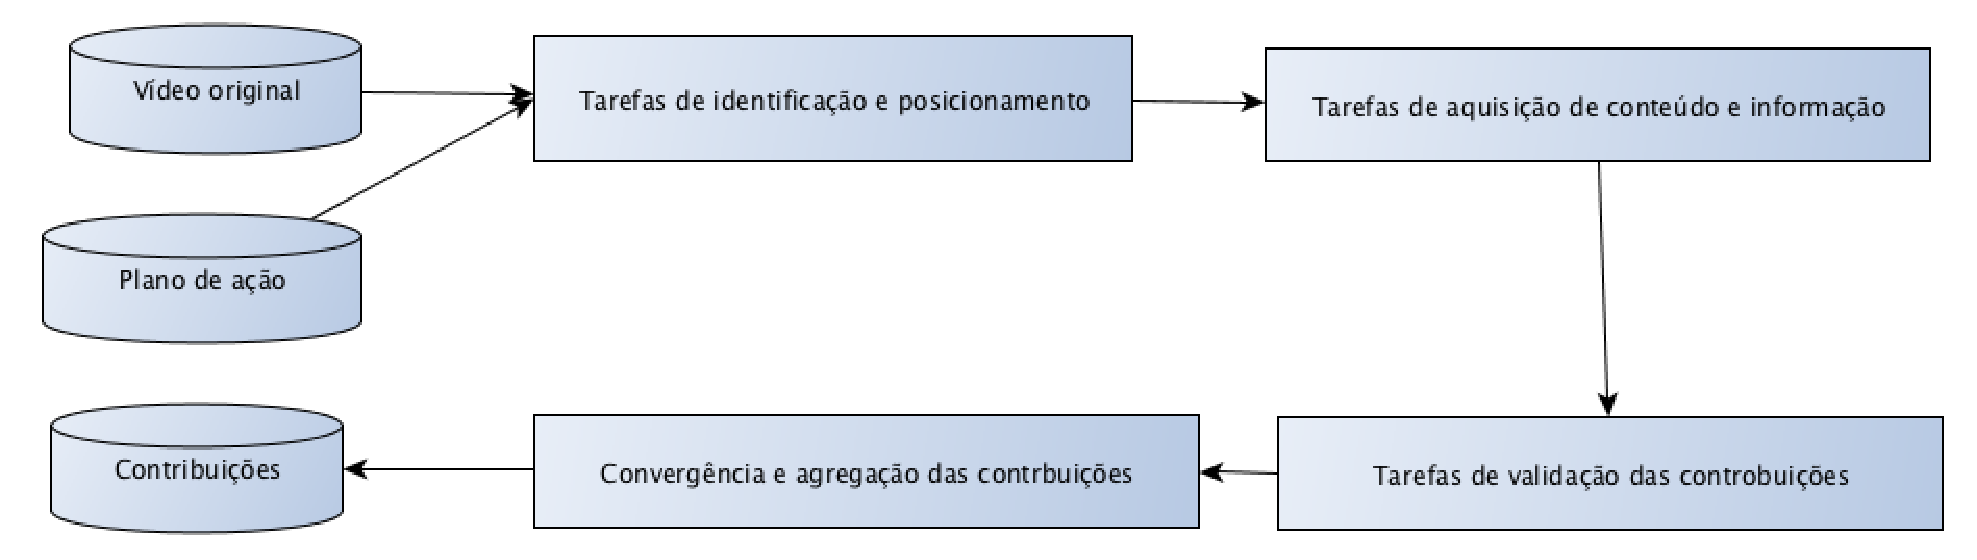
\includegraphics[width=.99\textwidth]{imagens/metodo/fase2_oa.eps}
\caption{Fase 2 do método}
\label{fig:metodo:fase2}
\end{figure}

Os três tipos de atividade, que foram modeladas como tarefas de anotação sobre o vídeo, são realizadas pelo Estudante. As tarefas são distribuídas entre eles de forma a coletar contribuições que possam cobrir todos os pontos identificados no plano de ação. Estes pontos dizem respeito aos tipos de ocorrência no vídeo sobre as quais se deseja coletar contribuições. De acordo com o plano de ação podem ser realizadas um, dois, ou os três tipos de tarefa. Entretanto, as atividades são realizadas na sequência em que aparecem na Figura~\ref{fig:metodo:fase2}. Desta forma é possível determinar onde estão as lacunas semânticas, coletar sugestões sobre como preenche-las, e avaliar quais delas mais satisfazem os estudantes.

Após se obter as contribuições necessárias para realizar a cobertura definida no plano de ação, são aplicadas técnicas de convergência e agregação para consolidar a base de contribuições que será utilizada para gerar o conteúdo complementar.



\subsection{Fase 3: Geração do Conteúdo Complementar}
A fase 3 tem inicio com a utilização de técnicas automáticas para gerar artefatos multimídia a partir de modelos previstos. O Sistema consulta o plano de ação, e utiliza as informações contidas na base consolidada de contribuições para instanciar os artefatos multimídia definidos no plano de ação.  

\begin{figure}[ht]
\centering
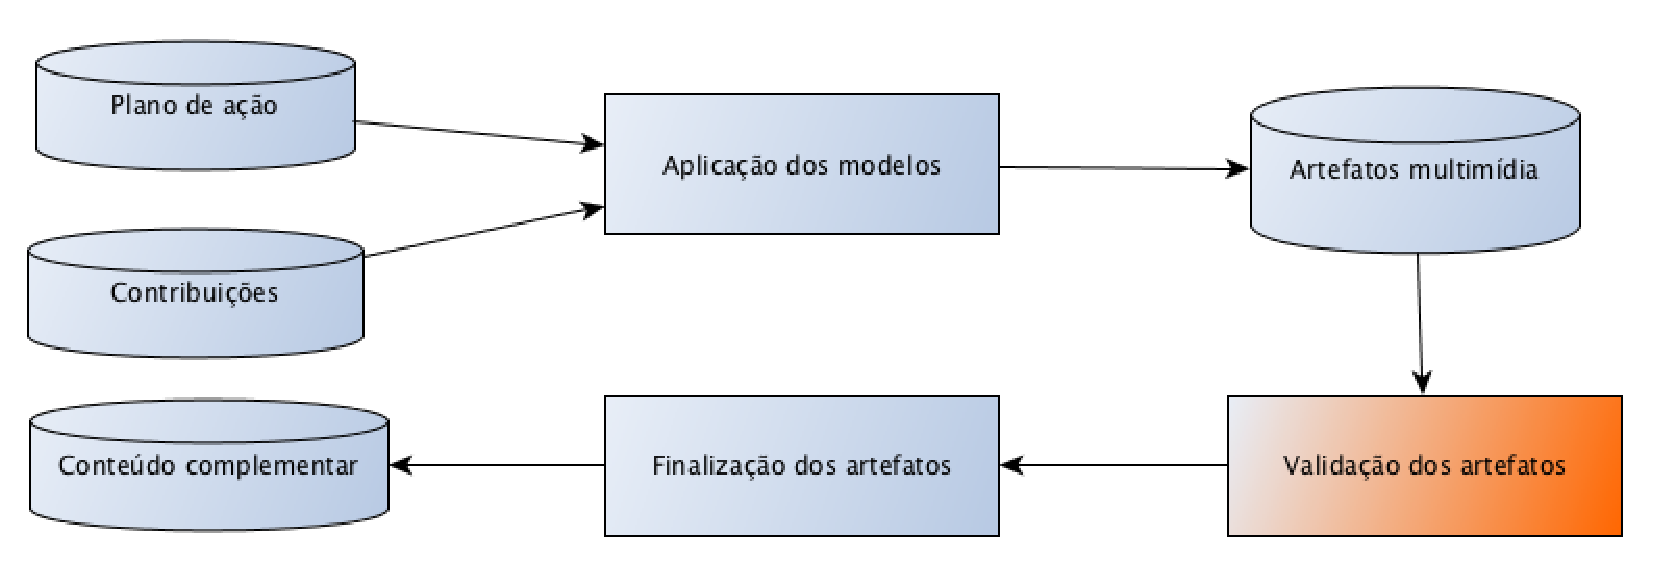
\includegraphics[width=.99\textwidth]{imagens/metodo/fase3_oa.eps}
\caption{Fase 3 do método}
\label{fig:metodo:fase3}
\end{figure}

Pode ser observado na Figura ~\ref{fig:metodo:fase3} que após gerados, os artefatos precisam ser validados. De acordo com o que foi definido no plano de ação, a validação pode ser feita pelo Iniciador, ou pelos Estudantes em uma abordagem semelhante a utilizada na fase 2. Uma vez validados, os artefatos são finalizados, ou seja, são formatados e adequados para serem agregados ao vídeo.



\subsection{Fase 4: Agregação do Conteúdo Complementar}
A fase 4 agrega o conteúdo complementar ao vídeo original de acordo com o plano de ação. Como pode ser visto na Figura~\ref{fig:metodo:fase4}, o conteúdo complementar é alinhado sobre a linha do tempo do vídeo original, para que possa ser apresentado de forma síncrona com o vídeo, nos momentos definidos na fase de contribuições.

\begin{figure}[ht]
\centering
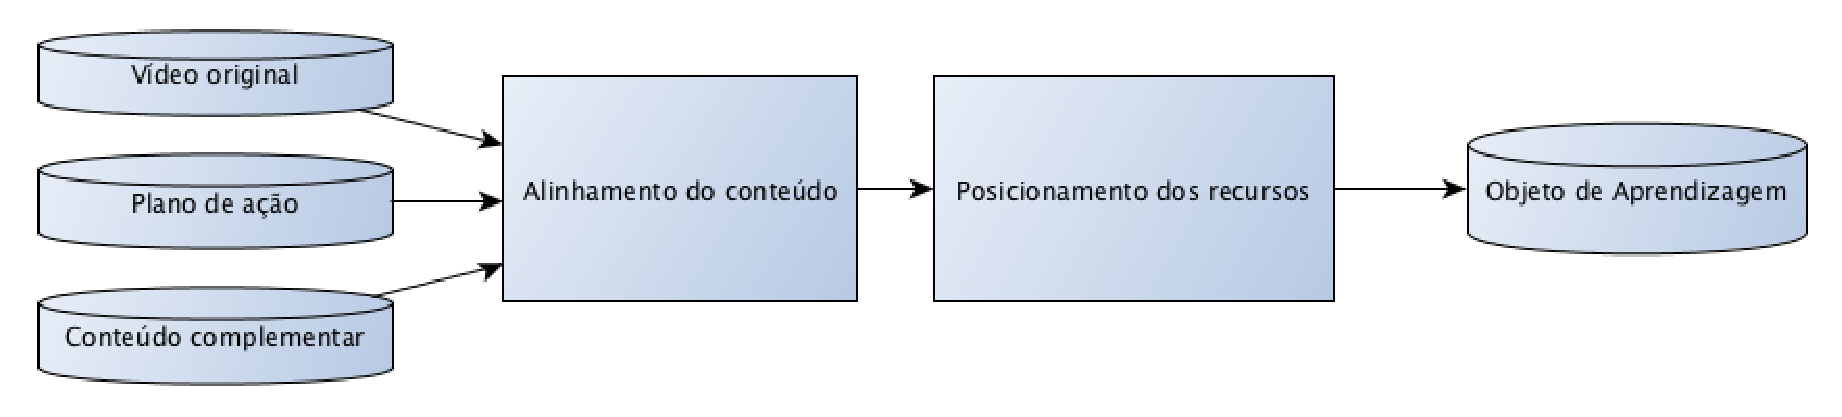
\includegraphics[width=.99\textwidth]{imagens/metodo/fase4_oa.eps}
\caption{Fase 4 do método}
\label{fig:metodo:fase4}
\end{figure}

Finalmente, cada artefato que compõe o conteúdo complementar é posicionado em relação ao vídeo de acordo com as definições do plano de ação, e desta forma o objeto de aprendizagem é finalizado.



\section{Ambiente de Apoio}
O método proposto neste trabalho é apoiado por um ambiente computacional formado por três componentes: módulo de colaboração, módulo de processamento, e módulo de apresentação. O fluxo de dados entre os componentes pode ser observado na Figura~\ref{fig:ambiente}.

\begin{figure}[ht]
\centering
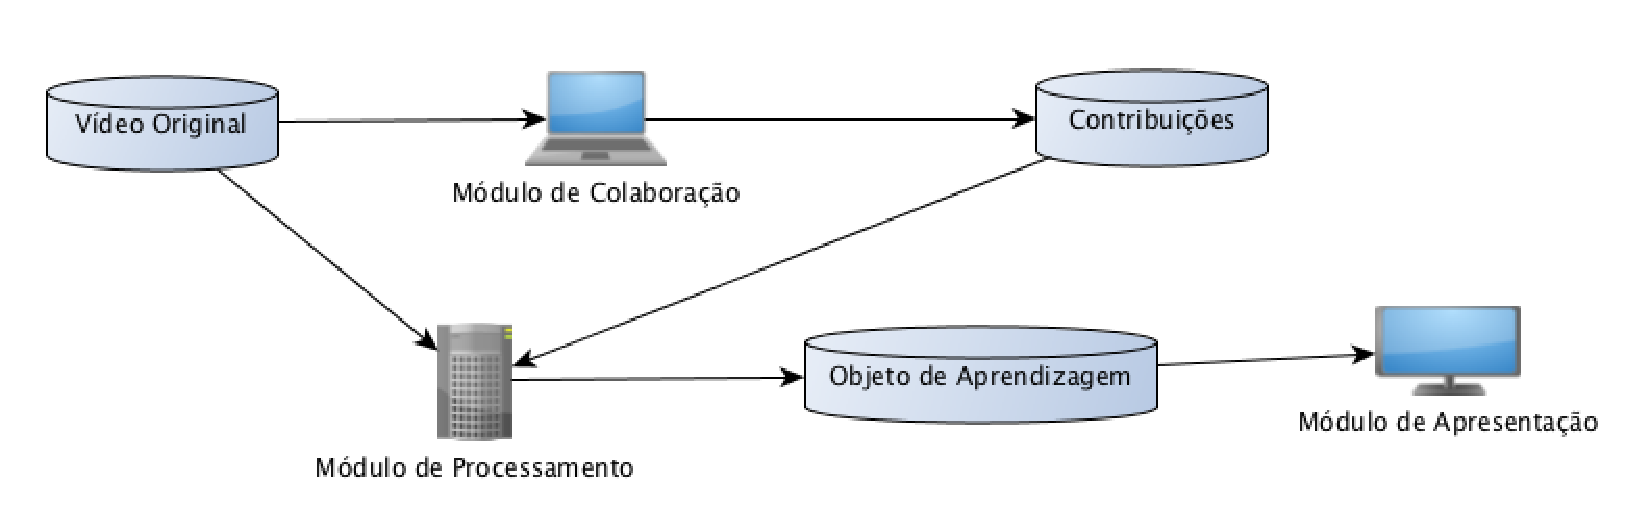
\includegraphics[width=.99\textwidth]{imagens/ambiente.eps}
\caption{Componentes do Ambiente de Apoio}
\label{fig:ambiente}
\end{figure}

O módulo de colaboração apoia as atividades de obtenção das informações necessárias para gerar o conteúdo complementar, a ser utilizado para enriquecer os vídeos. Por meio das ferramentas contidas nesse módulo, os estudantes podem contribuir de três maneiras: identificando lacunas semânticas, sugerindo conteúdos complementares para cobri-las, ou validando contribuições de outros estudantes. Esse módulo se baseia em uma abordagem crowdsourcing, que oferece suporte aos cenários de colaboração em escala massiva, além de propor formas eficientes de divisão e distribuição de tarefas, assim como de validação e agregação das contribuições. 

O módulo de processamento utiliza técnicas baseadas em modelos e funções paramétricas para gerar, a partir das contribuições dos estudantes, o conteúdo multimídia a ser agregado aos vídeos. Para este projeto foram selecionados três tipos de conteúdo: hiperlinks, caixas de texto e imagens. Os hiperlinks são inseridos em pontos do vídeo que requerem informação adicional, e apontam para outros vídeos ou páginas web com mais informações sobre os respectivos conceitos. As caixas de texto são utilizadas para contextualizar fatos e informações, para adicionar informações complementares, e para listar formas equivalentes para termos e expressões. As imagens são utilizadas para ajudar a explicar conceitos, apresentando desenhos, gráficos e fotografias que ajudem o estudante a compreender o conteúdo apresentado. 

O módulo de apresentação é utilizado para exibir os objetos de aprendizagem, com todas as funcionalidades necessárias para que o estudante possa interagir com eles. Adicionalmente esse módulo oferece funcionalidades que permitem aos estudantes fazerem recomendações, avaliações e sugestões de modificações nos objetos de aprendizagem.

\section{Estudo de Caso}
[DEFINIR NA REUNIÃO DE QUARTA-FEIRA 25/04 AS 9:30]

\section{Considerações Finais}
[ESCREVER APÓS O EXPERIMENTO]

\section{Agradecimentos}
Este trabalho é suportado pela Coordenação de Aperfeiçoamento de Pessoal de Nível Superior (CAPES) por meio do projeto nº 59/2014 – PGPTA.


\bibliographystyle{sbc}
\bibliography{referencias}

\end{document}
